\section{Related Work}
\label{related_work}
Generally speaking, there are two hashing methods categories: data-independent and data-dependent. Data-independent hashing methods usually generate a set of hash functions using randomization (without using any training data). In contrast,  data-dependent hashing methods usually are using unsupervised, supervised or semi-supervised learning techniques to generate the results. Here we are going to explain some relevant hashing mechanism to this report. 
\\
~
\\
\textbf{Operand locality}: Authors in \cite{compute-caches} proposed a mechanism for compute caches. In contrast to our problem, here the good results come out of locality of operands in the cache. Authors made some design choices in the cache organization such as defining banks that
have multiple sets each and added extra bits in address decoding for ``bank bits'' and ``block partition'' \cite{compute-caches}. This approach can be used to remember adjacent strides and scatter them into different cache lines.
\\
~
\\
\textbf{Using synthesis for a mapping algorithm}: In \cite{synthesis-map} authors implemented a synthesizing methodology to map p-nested for loop algorithms into linear arrays. The method was based on a set of formal conditions on the sequential algorithm and the feasible ``transformations'' on them. The result was promising given the time that this paper has published.
\\
~
\\
\textbf{Supervised hash algorithms}:

The authors in \cite{learning-hash} proposed a hashing method that is implemented using column generation based convex optimization. Considering a set of constraints, their proposed hashing method is capable of learning compact hash codes. Their Hash functions are learned iteratively using column generation.

In \cite{learning-index} authors showed that learned indexes outperforms traditional hash algorithms because utilizing the distribution of data being indexed can provide significant benefits. Figure \ref{fig:learned_index} shows how resistant their approach is to hash collisions in comparison to traditional hashing. 

\begin{figure}[h!]
	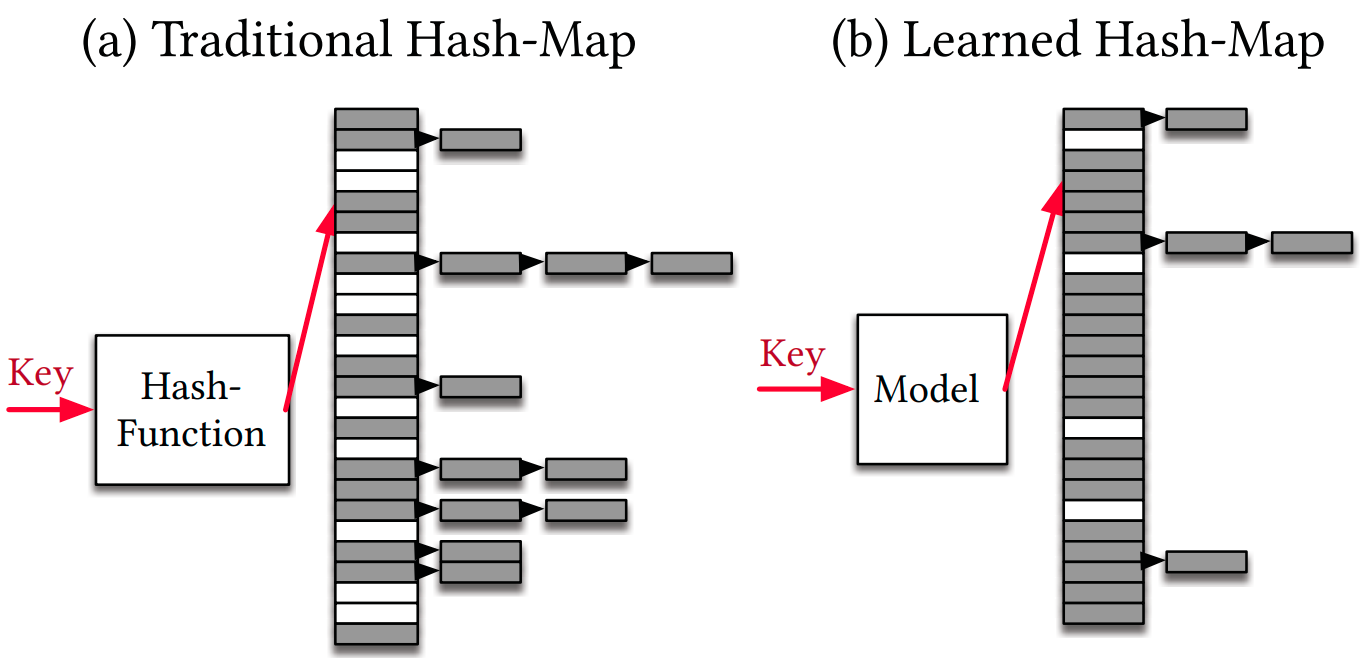
\includegraphics[scale=0.2]{figures/learned_index.png}
	\caption{Traditional Hash-map vs Learned Hash-map \cite{learning-index}}
	\label{fig:learned_index}
\end{figure}

\vspace{1mm}
\noindent
